%%%%%%%%%%%%%%%%%%%%%%%%%%%%%%%%%%%%%%%%%%%%%%%%%%%%%%%%%%%%%%%%%%%%%%%%%%%%%%%%
% event_selection.tex: Select of showering and tracking events:
%%%%%%%%%%%%%%%%%%%%%%%%%%%%%%%%%%%%%%%%%%%%%%%%%%%%%%%%%%%%%%%%%%%%%%%%%%%%%%%%
% cuts change to selection or requirement %
\chapter{Requirements and Efficiency}
\label{Chap:Efficiency}

In Sec. \ref{Sec:Acceptance}, the acceptance requirements for the \Z boson decays to be considered for this analysis were established as having at least one electron with $\pt > \SI{30}{GeV}$ and $|\eta| <2.1$, having a second electron with $\pt > \SI{20}{GeV}$ and $|\eta| <2.4$, and finally requiring the pair to have $\SI{60}{GeV}<\mee<\SI{120}{GeV}$. However, not every event which met those requirements when produced in the collider will be properly measured and reconstructed, and will be ``lost."


We use efficiency to describe the number of correct events lost for one reason or another. The efficiency is defined as the number of \Z events that decay to leptons with kinematic properties that have passed the acceptance requirements, divided by the number of events that should have passed all requirements ($\epsilon=\text{n}^{\text{obs.}}_{\text{pass}}/\text{n}^{\text{obs}}_{\text{total}}$). In order to accurately calculate the true distribution of \phistar, $\epsilon$ must be accurately calculated and applied.  

There are many reasons that an ``acceptable" electron may be rejected.  Even if the true parameters of the electron are within the window, if the measured values fall outside the acceptance window the event will be thrown out, such as if the true \pt of the electron was $\SI{21}{GeV}$ but the measurement yields $\SI{19}{GeV}$. Unfolding the distribution makes it possible to compensate for these effects. A second way for an electron to not be included is if for some reason the electron is not reconstructed. This can happen if the electron does not deposit energy in ECAL by falling into a crack between crystals or depositing all its energy in the tracker. An electron could also be rejected due to spatial overlap with other particles in the same event. For example, if a photon happens to deposit energy in the same crystal as the electron, the electron's energy measured by ECAL and the electron's momentum measured by the tracker will be incompatible. Due to this incompatibility, the reconstruction algorithm may reject the electron.   
\section{Requirements}
The efficiency is often lowered due to requirements to remove reconstructed electrons that are not produced from \Z decay. These background events can include photons that pair produce ($\gamma\rightarrow\xxpm{e}{e}$) inside the tracker, and  events that do not include an electron, such as a charged pion that interacts inside the ECAL depositing all its energy in a crystal. There can also be coincidence events, in which a charged particle leaves a track to a cluster that had a photon deposit energy.

Rather than have each analysis team pick every requirement completely independently, requirements are grouped into sets by the CMS Collaboration and studied centrally. These groups of requirements are designed to remove fake or unimportant electrons, such as electrons that are produced by a high energy particle interaction with the tracker, while keeping interesting electrons. The severity of these requirements is chosen depending on how important it is to remove backgrounds compared to how vital it is to not remove real electrons. This analysis uses two different sets of requirements, referred to as \EGTIGHT and \EGMEDIUM, with the more severe requirement being the \EGTIGHT. The specific requirements of \EGTIGHT and \EGMEDIUM are shown in Table \ref{table:eg_cuts}.
\begin{table}[ht]
    \centering
    \spacerows{1.2}
    \begin{center}
        \begin{tabular}{@{}l r r r r r@{}}
            \toprule
            \multirow{2}{*}{Variable}     & \multicolumn{2}{c}{\EGTIGHT} & \phantom{abc}   & \multicolumn{2}{c}{\EGMEDIUM} \\
            \cmidrule{2-3}
            \cmidrule{5-6}
            & \multicolumn{1}{c}{EB} & \multicolumn{1}{c}{EE} && \multicolumn{1}{c}{EB} & \multicolumn{1}{c}{EE} \\
            \midrule
            $\detain <$                   & 0.004     & 0.005     && 0.004     & 0.007 \\
            $\dphiin <$                   & 0.03      & 0.02      && 0.06      & 0.03 \\
            $\sigmaietaieta <$            & 0.01      & 0.03      && 0.01      & 0.03 \\
            $\HOverE <$                   & 0.12      & 0.10      && 0.12      & 0.10 \\
            $\dzero <$                    & 0.02      & 0.02      && 0.02      & 0.02 \\
            $\dz <$                       & 0.1       & 0.1       && 0.1       & 0.1 \\
            $|\ooeoop| <$                 & 0.05      & 0.05      && 0.05      & 0.05 \\
            $\pvtx <$                     & $10^{-6}$ & $10^{-6}$ && $10^{-6}$ & $10^{-6}$ \\
            $\nmiss \le$                  & 0         & 0         && 1         & 1 \\
            $\PFISO <$                    & 0.10      & 0.10      && 0.15      & 0.15 \\
            \bottomrule
        \end{tabular}
    \end{center}
    \caption[
        Identification and isolation requirements for \EGTIGHT and \EGMEDIUM.
    ]{
        Identification and isolation requirements for \EGTIGHT and \EGMEDIUM
        requirements in the ECAL barrel (EB) and ECAL endcap (EE).
    }
    \label{table:eg_cuts}
\end{table}
\subsection{Fake Electrons}
Many methods are used to lower the rate at which fake electrons are reconstructed. As mentioned, these fake electrons can have multiple sources, such as photons, pions, or even protons. One method to reduce the level of hadronic events being mislabeled as an electron is to use the ratio of the energy read out of HCAL in the area around where the hit was in ECAL, H/E. As mentioned earlier, electrons tend to deposit all their energy in ECAL, leading to a small value of H/E. In comparison, hadrons tend to travel through ECAL, keeping some of their energy until they get to HCAL, leading to a larger H/E value. This is shown in Fig. \ref{fig:HadronOverElectron}.

\begin{figure}[!htbp]
    \centering
    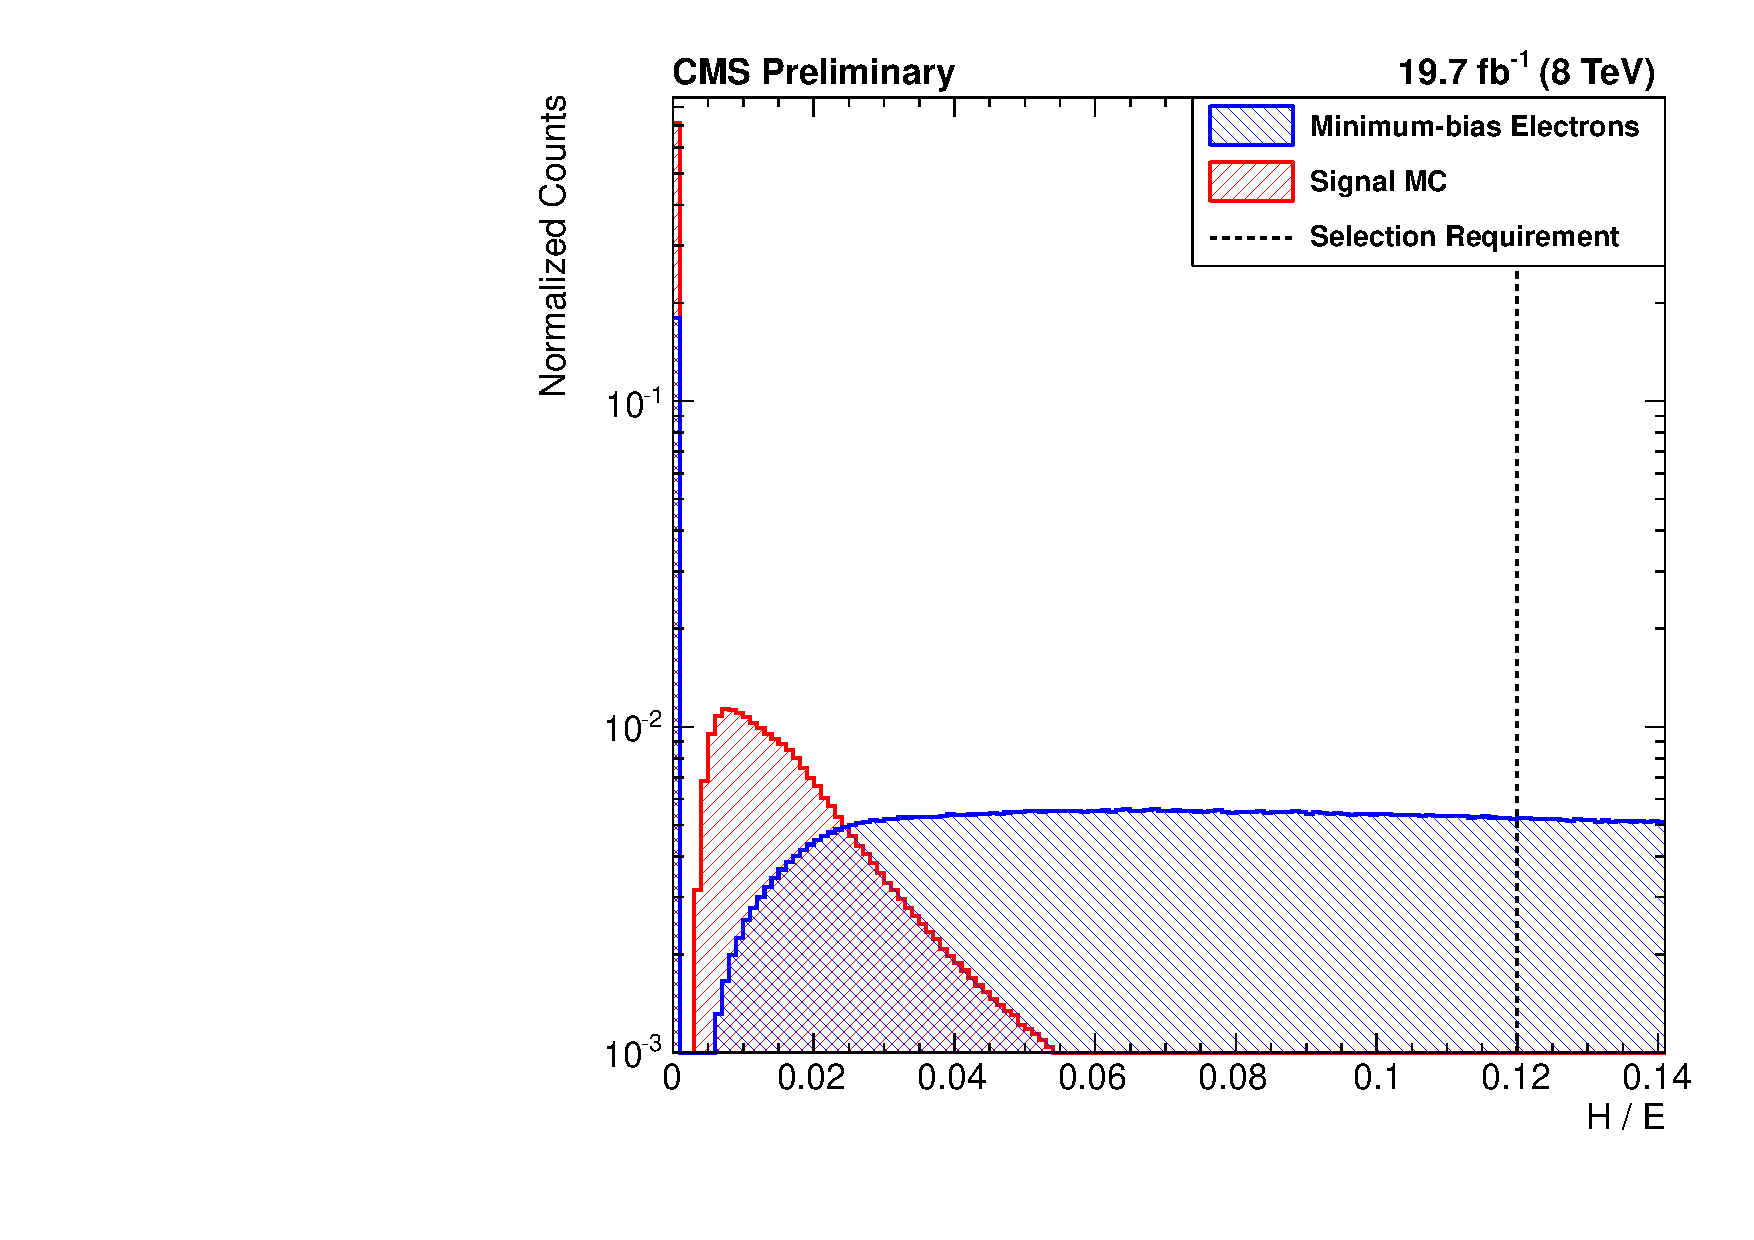
\includegraphics[width=\linewidth]{figures/EventSelection/AlexsEventSelectionFigures/e_reco_var_he.pdf}
    \caption[H/E comparison]{The H/E ratio of reconstructed electrons in a minimum bias sample compared to a \MADGRAPH \Ztoee sample. These electrons were required to be in the acceptance region, with \pt $>\SI{20}{GeV}$ and $|\eta|<2.4$. Electrons from the Z decay tend to not deposit much energy in the hadron calorimeter, with no events having a H/E above 6\%. In contrast the reconstructed electrons from the minumum bias sample have a relatively uniform distribution.}
    \label{fig:HadronOverElectron}
\end{figure}

If a hadron deposits all of its energy in ECAL, H/E discrimination will not work. A common cause of this is when a positively charged pion interacts with a neutron: 
\begin{equation}\label{eq:chargeExch}
    \pionplus+\neutron \rightarrow \pionzero+\proton\rightarrow 2\photon+\proton .
\end{equation}
This is referred to as charge exchange. Because of the short lifetime of the $\pionzero$, almost all of its energy is deposited in the crystal as two photons. This tends to lead to a larger shower than a single electron. Because of this, and the fact that hadron showers in general are larger than electron showers, it is possible for shower size requirements to effectively help differentiate the two. The shower width in the $\eta$(\sigmaietaieta) is used since the curvature of the electron in the magnetic field can widen its shower in the $\phi$ direction, but will not effect the shower shape in the $\eta$ direction.

Checking the consistency of the tracked particle's measured momentum value ($p$) vs the energy deposited in the cluster ($E$) can also be a useful measurement in removing fake electrons. Due to the tracker's increasing fractional uncertainty of $p$ at high momenta, these comparisons are done with their inverse, ($1/E-1/p$). For electrons this should be close to 0, while for hadrons that do not deposit all their energy in ECAL, this will be positive, and events caused by a coincidence can be either positive or negative values. Therefore both sets of selections, \EGTIGHT and \EGMEDIUM, include the requirement  $|1/E-1/p|<\SI{0.05}{GeV}^{-1}$. A plot comparing the $1/E-1/p$ of reconstructed electrons from a \Ztoee simulated sample to a minimum bias sample is shown in Fig \ref{fig:InverseEnMinusInverseMom}

\begin{figure}[!htbp]
    \centering
    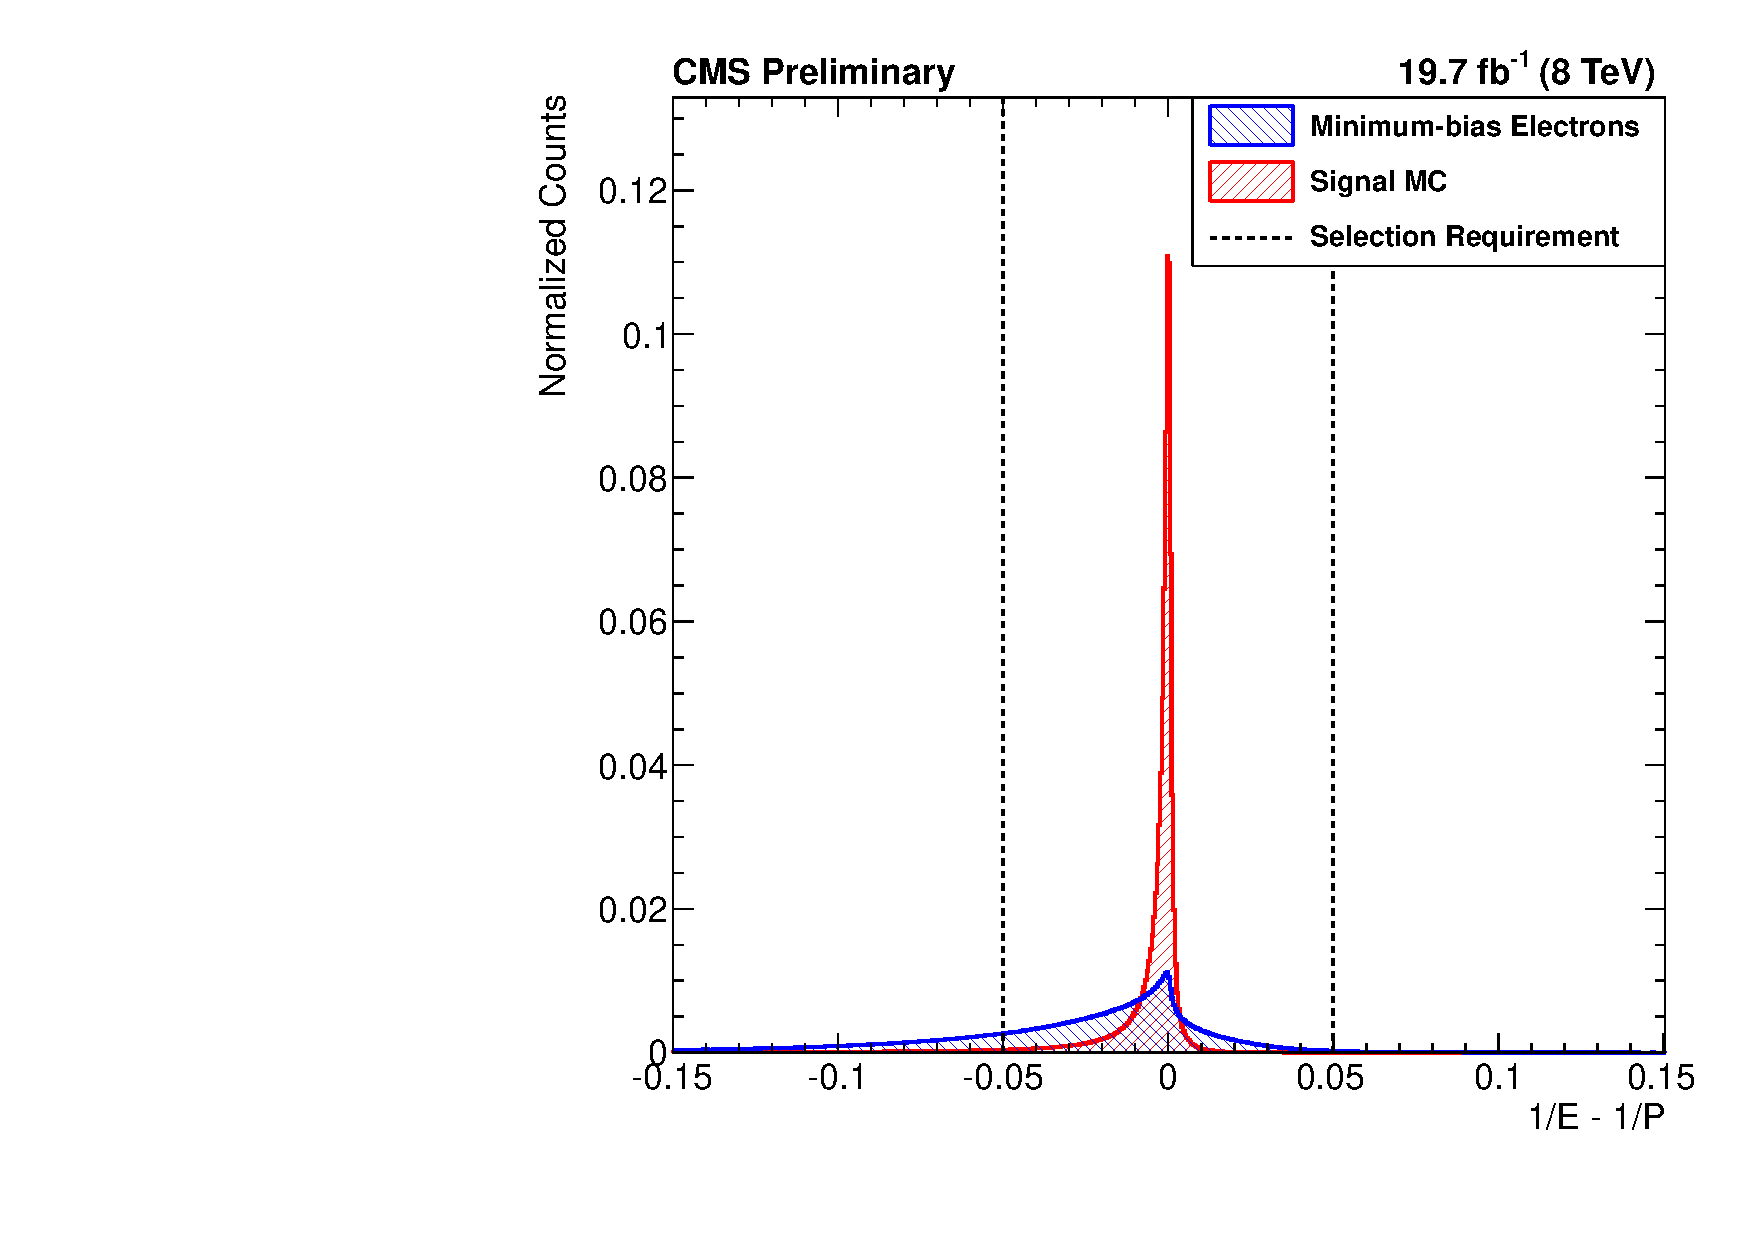
\includegraphics[width=\linewidth]{figures/EventSelection/AlexsEventSelectionFigures/e_reco_var_1oe_1op.pdf}
    \caption{The $1/E-1/p$ of reconstructed electrons in a minimum bias sample compared to a \MADGRAPH \Ztoee sample. These electrons were required to be in the acceptance region, with \pt $>\SI{20}{GeV}$ and $|\eta|<2.4$. For the signal sample almost all events are within 0.01 GeV$^{-1}$ of 0, while the minimum bias tail continues in both the negative and positive direction.}
    \label{fig:InverseEnMinusInverseMom}
\end{figure}
\subsection{Electrons from other sources}
Many processes other than \Z decay are capable of producing electrons. These electrons can also be suppressed by selection requirements, each of which may introduce an inefficiency.
\subsubsection{Electrons from Pair productions}
Pair production happens when a high energy photon interacts with a nucleus, creating an electron-positron pair, $\gamma\rightarrow\ee$. Due to the need for a nucleus, pair production tends to happen in the tracker, leading to two simple ways of rejecting these types of events.

The first way is by looking at the position of the electron's production vertex compared to the collision point. The second way is by looking at the track and how many layers it was detected in. Since on average, pair production happens after the photon travels through several layers, there will be many layers of the track in which the tracker does not see the electron. 
\subsubsection{Electrons from Jets}
During the production of a jet, it is possible for electrons to be produced through the decay of hadrons. These electrons are usually surrounded by other particles of all types. These other particles then deposit energy in ECAL and HCAL allowing the embedded electrons to be rejected by observing the area around the electron. For electrons produced by Z decay, not much energy is deposited around the electron. In contrast, jet produced electrons are accompanied by energy deposits over a wide range of space from the rest of the jet.

Isolation is defined as a ratio of the electron energy to all other energy around the electron event. Mathematically, in ECAL and HCAL, the isolation is defined as
\begin{equation}\label{eq:ECALIso}
    \ECALISO
    =
    \frac{\DeltaRSum{\EECAL-\ESC}}{\etElectron} ,
\end{equation}

\begin{equation}\label{eq:HCALIso}
    \HCALISO
    =
    \frac{\DeltaRSum{\EHCAL}}{\etElectron}.
\end{equation}
These variables attempt to find how much energy is deposited within a certain \DeltaR around the central crystal: $\DeltaR = \sqrt{\Delta\eta^2+\Delta\phi^2}$, where $\Delta\eta$ is the distance in $\eta$ from the central crystal, and $\Delta\phi$ is the distance in $\phi$. By subtracting $\ESC$, the energy in the super-cluster, in the calculation of \ECALISO, the contribution of the electron itself is removed from the isolation calculation. Because almost none of the energy from the electron is deposited in HCAL, no subtraction is required for \HCALISO. The last type of isolation used is the particle flow isolation, defined as 

\begin{equation}\label{eq:ECALIso2}
    \PFISO
    =
    \frac{\DeltaRSum{(\ptTrack+\EHCAL+\EECAL-\ESC-\ptElectron-0.3^2\pi\rho)}}{\ptElectron}.
\end{equation}
This isolation variable includes two new variables: \ptTrack, the measured $\pt$ of the tracks surrounding the central crystal, and $\rho$, a variable that helps compensate for pileup. Each time a bunch crosses, multiple protons interact. Most of these interactions do not produce any heavy particles, but they do cause a spray of low energy light particles leading to a deposit of energy all over the detector.  The $\rho$ is calculated for each event by counting the particles that did not end up in a jet.


\section{Measuring Efficiency using Data}
\label{sec:Measuing_Efficiency}
 The efficiency of requirements, such as \EGTIGHT and \EGMEDIUM,  can be calculated based on simulated samples because the simulation has access to both the generator level electrons as well as the reconstructed level. However, there are differences between reconstructed particles in the simulation and reality that must be compensated for. This requires knowledge of the data efficiency, which is tricky to do since it requires a sample of pure electrons that we are interested in. Because the selections are to remove the background, a different method is required to remove the background from the sample in order to find the efficiency of the selections on data. The popular method to do this is the tag-and-probe method. The tag-and-probe method requires an event to have one reconstructed electron that passes very stringent requirements. This electron is known as the tag. This tag electron is then matched to another possible electron object. If the pair has an invariant mass close to the Z mass it is very likely that this was an electron produced from a Z decay. The electron matched to the tag electron is called the probe. These probes are used to calculate the efficiency of the selections on data. This is necessary due to differences between the simulated detector and the real detector, leading to different efficiencies for the data and the simulation. A scale factor, which is used to compensate for these differences, is defined as: 
\begin{equation}\label{eq:ScaleFactor}
    SF
    =
    \frac{\epsilon_{Data}}{\epsilon_{simulation}}.
\end{equation}
%The second type of efficiency is the efficiency of events in each \phistar bin. This is required to correct the final \phistar distribution. This other efficiency was defined in Chapter \ref{Chapt:Data_Anaylysis_Stratagy}.
\subsection{Tag-and-probe requirements}

\subsubsection{Single Electron Trigger}
The electron data set that was used in this analysis was created with a ``single electron trigger," \SingleElectronTrigger, and was taken from 2012 CMS data.  This trigger was created to save events that contain at least one electron with $\pt>\SI{27}{GeV}$. This trigger was chosen due to its similarity to the single muon trigger, allowing direct comparisons to be made between \Ztoee and \Ztomumu data sets.

The efficiency of the trigger that was used to create the  \SingleElectronTrigger was measured using the tag-and-probe method on the data set itself. In order to be considered, an event must pass four requirements:
\begin{itemize}
    \item Two electrons with $\pt>\SI{30}{GeV}$ and $|\eta|<2.1$
    \item Both Electrons must pass the \EGTIGHT requirement
    \item The invariant mass of the system falls in the range of $\SI{60}{GeV}<m_{\text{ee}}<\SI{120}{GeV}$
    \item The tag electron is required to be close to an HLT trigger object with $\Delta R <  0.3$.
\end{itemize}
 If an event has more then two electrons satisfying these requirements it is not considered. A probe is considered passing if it matches with an HLT trigger object with $\Delta R <  0.3$. Because of the similar requirements on the tag and the probe, if the probe passes, then it can also be the tag, causing these events to be counted as two passes, while an event that the probe fails is counted as one fail. The efficiency for simulation and data is shown in Tables \ref{table:trigger_eff_data} and \ref{table:trigger_eff_mc}.

\begin{table}[t]
    \centering
    \spacerows{1.5}
    \begin{center}
        \begin{tabular}{@{}l r r r r r@{}}
            \toprule
            $\eta$ & \GeVRange{30}{40} & \GeVRange{40}{50} & \GeVRange{50}{70} & \GeVRange{70}{250}  \\
            \midrule
            \numrange{-2.1}{-2} & $0.741^{+0.003}_{-0.003}$ & $0.773^{+0.003}_{-0.003}$ & $0.780^{+0.005}_{-0.005}$ & $0.79^{+0.01}_{-0.01}$  \\
            \numrange{-2}{-1.556} & $0.734^{+0.001}_{-0.001}$ & $0.772^{+0.001}_{-0.001}$ & $0.786^{+0.002}_{-0.002}$ & $0.792^{+0.005}_{-0.005}$  \\
            \numrange{-1.556}{-1.442} & $0.725^{+0.003}_{-0.003}$ & $0.821^{+0.002}_{-0.002}$ & $0.809^{+0.004}_{-0.004}$ & $0.848^{+0.010}_{-0.010}$  \\
            \numrange{-1.442}{-0.8} & $0.8930^{+0.0005}_{-0.0005}$ & $0.9396^{+0.0003}_{-0.0004}$ & $0.9509^{+0.0006}_{-0.0006}$ & $0.966^{+0.001}_{-0.001}$  \\
            \numrange{-0.8}{0} & $0.9213^{+0.0004}_{-0.0004}$ & $0.9528^{+0.0002}_{-0.0002}$ & $0.9601^{+0.0004}_{-0.0004}$ & $0.9692^{+0.0010}_{-0.0010}$  \\
            \numrange{0}{0.8} & $0.9174^{+0.0004}_{-0.0004}$ & $0.9473^{+0.0003}_{-0.0003}$ & $0.9561^{+0.0004}_{-0.0004}$ & $0.963^{+0.001}_{-0.001}$  \\
            \numrange{0.8}{1.442} & $0.8964^{+0.0005}_{-0.0005}$ & $0.9424^{+0.0003}_{-0.0003}$ & $0.9533^{+0.0006}_{-0.0006}$ & $0.966^{+0.001}_{-0.001}$  \\
            \numrange{1.442}{1.556} & $0.714^{+0.003}_{-0.003}$ & $0.823^{+0.002}_{-0.002}$ & $0.827^{+0.004}_{-0.004}$ & $0.861^{+0.009}_{-0.010}$  \\
            \numrange{1.556}{2} & $0.758^{+0.001}_{-0.001}$ & $0.800^{+0.001}_{-0.001}$ & $0.811^{+0.002}_{-0.002}$ & $0.823^{+0.005}_{-0.005}$  \\
            \numrange{2}{2.1} & $0.764^{+0.003}_{-0.003}$ & $0.792^{+0.002}_{-0.002}$ & $0.797^{+0.005}_{-0.005}$ & $0.82^{+0.01}_{-0.01}$  \\
            \bottomrule
        \end{tabular}
    \end{center}
    \caption{
        The electron trigger efficiency in data.
    }
    \label{table:trigger_eff_data}
\end{table}

\begin{table}[ht]
    \centering
    \spacerows{1.5}
    \begin{center}
        \begin{tabular}{@{}l r r r r r@{}}
            \toprule
            $\eta$ & \GeVRange{30}{40} & \GeVRange{40}{50} & \GeVRange{50}{70} & \GeVRange{70}{250}  \\
            \midrule
            \numrange{-2.1}{-2} & $0.734^{+0.004}_{-0.004}$ & $0.769^{+0.004}_{-0.004}$ & $0.771^{+0.008}_{-0.008}$ & $0.76^{+0.02}_{-0.02}$  \\
            \numrange{-2}{-1.556} & $0.736^{+0.002}_{-0.002}$ & $0.768^{+0.002}_{-0.002}$ & $0.779^{+0.003}_{-0.003}$ & $0.789^{+0.008}_{-0.008}$  \\
            \numrange{-1.556}{-1.442} & $0.791^{+0.004}_{-0.004}$ & $0.847^{+0.003}_{-0.003}$ & $0.850^{+0.006}_{-0.006}$ & $0.87^{+0.01}_{-0.02}$  \\
            \numrange{-1.442}{-0.8} & $0.9395^{+0.0006}_{-0.0006}$ & $0.9612^{+0.0004}_{-0.0004}$ & $0.9690^{+0.0007}_{-0.0008}$ & $0.980^{+0.002}_{-0.002}$  \\
            \numrange{-0.8}{0} & $0.9469^{+0.0005}_{-0.0005}$ & $0.9670^{+0.0003}_{-0.0003}$ & $0.9745^{+0.0005}_{-0.0005}$ & $0.982^{+0.001}_{-0.001}$  \\
            \numrange{0}{0.8} & $0.9466^{+0.0005}_{-0.0005}$ & $0.9665^{+0.0003}_{-0.0003}$ & $0.9739^{+0.0005}_{-0.0006}$ & $0.982^{+0.001}_{-0.001}$  \\
            \numrange{0.8}{1.442} & $0.9364^{+0.0007}_{-0.0007}$ & $0.9597^{+0.0004}_{-0.0004}$ & $0.9668^{+0.0008}_{-0.0008}$ & $0.979^{+0.002}_{-0.002}$  \\
            \numrange{1.442}{1.556} & $0.779^{+0.004}_{-0.005}$ & $0.841^{+0.003}_{-0.003}$ & $0.842^{+0.006}_{-0.006}$ & $0.86^{+0.02}_{-0.02}$  \\
            \numrange{1.556}{2} & $0.749^{+0.002}_{-0.002}$ & $0.786^{+0.002}_{-0.002}$ & $0.798^{+0.003}_{-0.003}$ & $0.810^{+0.008}_{-0.008}$  \\
            \numrange{2}{2.1} & $0.737^{+0.004}_{-0.004}$ & $0.769^{+0.004}_{-0.004}$ & $0.779^{+0.007}_{-0.008}$ & $0.82^{+0.02}_{-0.02}$  \\
            \bottomrule
        \end{tabular}
    \end{center}
    \caption{
        The electron trigger efficiency in \MADGRAPH simulation.
    }
    \label{table:trigger_eff_mc}
\end{table}
Since the single electron trigger only needs one electron to trigger it, there are not two scale factors for each electron, but rather one scale factor based on whether either the leading($\epsilon_\text{L}$) or trailing($\epsilon_\text{T}$) electron triggers the HLT:
\begin{equation}
    SF_{\text{L or T}}
    =
    \frac{1-(1-\epsilon_\text{L}^{\text{Data}})(1-\epsilon_\text{T}^{\text{Data}})}{1-(1-\epsilon_\text{L}^{\text{simulation}})(1-\epsilon_\text{T}^{\text{simulation}})}.
\end{equation}
In the case where the trailing electron either has $\pt<\SI{30}{GeV}$ or $|\eta|>2.1$ then $\epsilon_\text{T}^{\text{Data}}=\epsilon_\text{T}^{\text{simulation}}=0$.

\subsubsection{Electron Reconstruction Efficiency}
The electron GSF reconstruction scale factors are centrally produced \cite{GSF_Scale_Factors_Twiki}. In order for an electron to be reconstructed, a track must be matched to a super cluster in ECAL. If the electron's energy is either not deposited in the crystal or deposited in dead crystals in the detector, the electron will not be seen with ECAL. Since this method lacks an energy deposit, there is nothing to match to the tag electron to act as the probe. For this reason, the loss of efficiency due to super clusters failing to form is calculated from simulation.  The efficiency and scale factor that come from matching super clusters to tracks is done using a data sample that was created with a special tag-and-probe trigger, \TnPTrigger. This trigger requires one electron with $\pt>\SI{20}{GeV}$, passing very tight ID and isolation requirements. By requiring $\mee>\SI{50}{GeV}$ a very lax requirement can be placed on the other electron's transverse energy ($\ET>\SI{4}{GeV}$). In order to reject events that are poorly reconstructed, good events are required to have all the reconstructed particles be well-balanced transversely, with the particle flow missing transverse energy being less than 20 GeV.  Reconstructed tag electrons are required to match spatially to the $\EGTIGHT$ trigger electron. This reconstructed electron is then required to pass $\EGTIGHT$, as well as $\pt>\SI{25}{GeV}$ and $\eta<2.5$. Electrons that fall in the gap between the ECAL barrel and endcap, $1.4442<|\eta|<1.566$,  are  rejected. The super-cluster is required to have a tracker isolation of  $<0.15$. The simulation requires that the reconstructed tag electron matches with a generated electron, with $\DeltaR < 0.2$.
For simulation, $\text{n}^{\text{obs.}}_{\text{pass}}$ and $\text{n}^{\text{obs}}_{\text{total}}$ are the counts of the probe that pass and total probes, respectively. For data, the background is compensated for by first separating events by the probe $\pt$ and $\eta$, and creating a distribution of the dielectron invariant mass. This distribution is then fit with a Gaussian-smeared $\Ztoee$ simulation sample added to an exponential that represents the background. These fits were used to calculate the  $\text{n}^{\text{obs.}}_{\text{pass}}$ and $\text{n}^{\text{obs}}_{\text{total}}$ that were used to calculate the efficiency of the data and the scale factors shown in Table~\ref{table:gsf_scale_factor}.



\begin{table}[ht]
    \centering
    \spacerows{1.5}
    \begin{center}
        \begin{tabular}{@{}l r r r r@{}}
            \toprule
            $|\eta|$                 & \GeVRange{20}{30}                  & \GeVRange{30}{40}                  & \GeVRange{40}{50}                  & $> \SI{50}{\GeV}$ \\
            \midrule
            \numrange{0.0}{0.8}      & $\effstatsys{0.982}{0.003}{0.012}$ & $\effstatsys{0.988}{0.001}{0.008}$ & $\effstatsys{0.990}{0.001}{0.004}$ & $\effstatsys{0.990}{0.001}{0.004}$ \\
            \numrange{0.8}{1.4442}   & $\effstatsys{0.993}{0.002}{0.012}$ & $\effstatsys{0.993}{0.001}{0.008}$ & $\effstatsys{0.993}{0.001}{0.004}$ & $\effstatsys{0.991}{0.001}{0.004}$ \\
            \numrange{1.4442}{1.566} & $\effstatsys{1.016}{0.012}{0.020}$ & $\effstatsys{0.985}{0.004}{0.009}$ & $\effstatsys{0.987}{0.004}{0.004}$ & $\effstatsys{0.974}{0.009}{0.006}$ \\
            \numrange{1.566}{2.0}    & $\effstatsys{0.988}{0.003}{0.012}$ & $\effstatsys{0.993}{0.002}{0.008}$ & $\effstatsys{0.992}{0.001}{0.004}$ & $\effstatsys{0.990}{0.003}{0.004}$ \\
            \numrange{2.0}{2.5}      & $\effstatsys{1.002}{0.004}{0.012}$ & $\effstatsys{1.004}{0.002}{0.008}$ & $\effstatsys{1.005}{0.002}{0.004}$ & $\effstatsys{0.998}{0.004}{0.004}$ \\
            \bottomrule
        \end{tabular}
    \end{center}
    \caption[
        Scale factors for GSF electron reconstruction.
    ]{
        Scale factors for GSF electron reconstruction. The upper uncertainty listed
        is statistical, the lower is systematic.
    }
    \label{table:gsf_scale_factor}
\end{table}




\subsection{\texorpdfstring{\phistar}{Phistar} efficiency}



The overall efficiency for the signal events in data can be calculated using a simulated sample by taking the previously calculated scale factors into account:
\begin{equation}
   \epsilon_i
   =
   \frac{\sum\limits_{obs}SF(l_1,l_2)}{n_i^{total}}
\end{equation}
Here, rather then using the number of observed events in the simulation directly, $n_i^{obs}$, each observed event uses $SF(l_1,l_2)$, which is the product of all applicable scale factors, and used as a weight to calculate the $\epsilon_i$ of data from simulated samples. 

%%%%%%%%%%%%%%%%%%%%%%%%%%%%%%%%%%%%%%%%%%%%%%%%%%%%%%%%%%%%%%%%%%%%%%%%%%%%%%%%

%%%%%%%%%%%%%%%%%%%%%%%%%%%%%%%%%%%%%%%%%%%%%%%%%%%%%%%%%%%%%%%%%%%%%%%%%%%%%%%%
